\chapter{Estado del arte}
\label{ch:estado-del-arte}

En este capítulo se realizará un análisis de diversas tecnologías y soluciones desarrolladas por diferentes empresas o comunidades que se relacionan con el tema propuesto en esta memoria. Todos estos componentes, tecnologías y herramientas comparten el objetivo de crear sistemas como los que queremos llevar a estudio, y vamos a observar que juntos conforman capas para formar otras herramientas que se verán más adelante. Se proporcionará una descripción concisa de cada tecnología, destacando sus características principales, y se analizará el estado de madurez que estas tienen en la actualidad. Este análisis permitirá situar nuestro análisis en unas condiciones específicas con unas tecnologías predefinidas.

\section{Introducción a las Tecnologías de Contenedores y Microservicios}

\subsection{Contenedores}

Los contenedores, pese a su gran auge en popularidad en los últimos años, son un concepto que se remonta a 1979 y a UNIX V7, donde se introdujo por primera vez el concepto de aislamiento de procesos. El concepto de contenedor más extendido a día de hoy, como espacios virtualizados aislados de un sistema operativo que permiten el despliegue de aplicaciones de manera reproducible y aislada, lo introdujo Docker en 2013, y tiene una estructura como la que podemos ver en la Figura \ref{fig:container-engine}. A día de hoy, Docker es el sistema más usado para el uso de contenedores en el mundo.

\begin{figure}[h!]
    \centering
    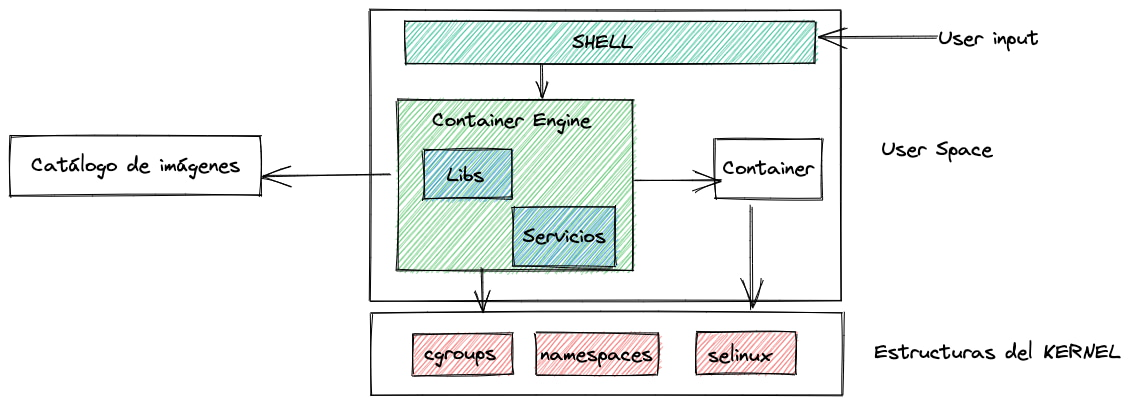
\includegraphics[width=1\linewidth]{figures/container-engine.jpg}
    \caption{Esquema de un motor de contenedores}
    \label{fig:container-engine}
\end{figure}


\subsection{Docker}

Docker nació como una herramienta de código libre. Permite a los desarrolladores empaquetar aplicaciones en contenedores, lo que facilita su despliegue y escalabilidad en diferentes entornos, desde máquinas locales hasta nubes públicas y privadas.

En el ámbito de la virtualización, Docker se ha establecido como una solución 
eficiente frente a las máquinas virtuales tradicionales, ofreciendo una mayor optimización de recursos y un despliegue más rápido de aplicaciones. Las empresas y desarrolladores valoran Docker por su simplicidad, portabilidad y la capacidad de aislar y ejecutar procesos de manera independiente, lo que mejora el uso de la infraestructura y mantiene la seguridad.

En 2017, el motor de Docker conocido como Docker Engine se dividió en varias partes de código libre, entre las que destacamos el Proyecto Moby y Containerd. El Proyecto Moby es un proyecto de software libre que permite a otros desarrolladores crear gestores de contenedores basados en los recursos que el mismo Docker usa para funcionar, y que cumple con la Open Container Iniciative (OCI). Containerd es un \textit{runtime} de contenedores de alto nivel que liberó Docker que permite correr contenedores y que es altamente customizable.


\begin{figure}[h!]
    \centering
    
\includegraphics[width=0.5\linewidth]{figures/Docker-Logo.png}
    \caption{Logo de Docker}
    \label{fig:Docker-Logo}
\end{figure}


\subsection{Containerd}

Containerd es un proyecto de código abierto que proporciona un entorno de ejecución de contenedores enfocado en la simplicidad, robustez y portabilidad. Nació en 2016 como parte de Docker, pero en 2017 se convirtió junto con Moby en un proyecto independiente que fue adoptado por la Cloud Native Computing Foundation (CNCF).

Está diseñado para ser menos complejo que Docker, proporcionando solo las funcionalidades básicas necesarias para ejecutar contenedores, aunque soporta por defecto las imágenes de Docker. Además, debido a su naturaleza menos compleja, se centraron en que customizable por medio de \textit{shims}. Un \textit{shim} es un proceso ligero que actúa como intermediario entre containerd y el proceso del contenedor en sí. Su función principal es gestionar la vida del proceso del contenedor, asegurando que este pueda continuar ejecutándose incluso si el proceso principal de containerd se detiene. Son estos shims los que permiten que podamos ejecutar WebAssembly en contenedores, como hablaremos más adelante.

\begin{figure}[h!]
    \centering
    
\includegraphics[width=0.5\linewidth]{figures/containerd-horizontal-color.png}
    \caption{Logo de Containerd}
    \label{fig:Containerd-Logo}
\end{figure}

\subsection{Kubernetes}

Kubernetes es un sistema de orquestación de contenedores de código abierto lanzado en 2014 por Google, que también forma parte de la CNCF. Se ha convertido en el estándar de facto para la orquestación de contenedores, con una adopción masiva en la industria, que ofrece una plataforma portable y extensible para desplegar tus aplicaciones. Entre sus mayores virtudes, cuenta con que es automatizable y que se configura de manera declarativa, ya que basa su configuración en \textit{Infrastructure as Code} (IaaC), lo que permite a sus usuarios especificar el estado deseado de las aplicaciones y servicios a desplegar de manera muy sencilla.

Este proyecto cuenta con el respaldo de muchas de las empresas más grandes del sector, que sustentan la mayor parte de operaciones sobre Kubernetes, y en una base de contribuidores particulares muy activa y en constante crecimiento.

Kubernetes usa como entorno de ejecución de contenedores a Containerd, a lo que hace que se abra la posibilidad de desplegar módulos de WebAssembly en él para aprovechar sus virtudes haciendo uso del shim de containerd más popular para ejecutar contenedores basados en WASM: RunWasi.

\begin{figure}[h!]
    \centering
    
\includegraphics[width=0.5\linewidth]{figures/kubernetes-logo.png}
    \caption{Logo de Kubernetes}
    \label{fig:kubernetes-logo}
\end{figure}

\section{WebAssembly (WASM) y su Evolución}

\subsection{WebAssembly}

WebAssembly (WASM) es una tecnología creada por el W3C que permite ejecutar código de bajo nivel en navegadores web con un rendimiento cercano al nativo. Nació en 2015, pero no fue hasta 2020 que el W3C lo reconoció como uno de los lenguajes estándar de «la web». Funciona como una capa de abstracción entre el código fuente y la plataforma subyacente, lo que significa que puedes escribir código en lenguajes como C++, Rust o incluso Python, y luego compilarlo a un formato binario optimizado que puede ser ejecutado directamente por el navegador. Cuando WebAssembly es ejecutado en el navegador, este lo hace en un entorno aislado dentro del navegador. Debido a que hay algunas características que siguen en fases tempranas de desarrollo, como el soporte de \textit{garbage collector}, hay ciertos lenguajes que no tienen soporte, como puede ser Java.

El resultado de las compilaciones a WASM da como resultado módulos de WebAssembly, que pueden ser usados de dos formas: insertado en el navegador a través de JavaScript, que es la forma de uso que principalmente se pensó para ello; o en contenedores aprovechando las características de los shims de Containerd, además de la WebAssembly System Interface (WASI).

\begin{figure}[h!]
    \centering
    
\includegraphics[width=0.5\linewidth]{figures/WebAssembly-Logo.png}
    \caption{Logo de WebAssembly}
    \label{fig:WebAssembly-Logo}
\end{figure}

\subsection{WebAssembly System Interface}

WebAssembly System Interface (WASI) es un conjunto de especificaciones de API estándar para software compilado al estándar WebAssembly del W3C. Está diseñado para aplicaciones que pueden ser compiladas a Wasm desde cualquier lenguaje y que pueden ejecutarse en cualquier lugar, desde navegadores hasta nubes y dispositivos integrados. En la actualidad, WASI ha tenido dos lanzamientos importantes conocidos como 0.1 y 0.2. Estas versiones son a veces referidas como \textit{Preview 1} y \textit{Preview 2}, o \textit{P1} y \textit{P2}. Busca mantener los principios clave de WebAssembly: portabilidad y seguridad.

Para comenzar con WASI, hay varios entornos de ejecución que lo soportan, incluyendo Wasmtime, WAMR, WasmEdge, wazero, Wasmer, wasmi y wasm3. Cada uno de estos entornos tiene diferentes áreas de enfoque, como WAMR que se enfoca en IoT, dispositivos embebidos o edge computing, o WasmEdge que se enfoca en el lado del servidor y en la ejecución de grandes modelos de lenguaje de inteligencia artificial.

WASI ha permitido la ejecución de código fuera del entorno del navegador, de una similar a como Node.js lo hizo con JavaScript. Esto ha hecho que podamos usar WebAssembly en entornos para los que inicialmente no estaba pensado, como contenedores y sistemas con arquitecturas basadas en microservicios.

\begin{figure}[h!]
    \centering
    
\includegraphics[width=0.5\linewidth]{figures/wasi.png}
    \caption{Logo de WASI}
    \label{fig:wasi-logo}
\end{figure}

\section{Aplicaciones de WebAssembly en Arquitecturas Basadas en Microservicios y Serverless}

\subsection{Implementación en contenedores}

Como hemos mencionado antes, la llegada de WASI, sobre todo en su P2, ha hecho viable la utilización de WebAssembly dentro de contenedores. Podemos usar esta tecnología para otorgar a los contenedores una capa extra de eficiencia y seguridad. WasmEdge es un runtime optimizado para ejecutar WebAssembly en entornos de contenedores como Docker. Este enfoque promete mejorar el rendimiento, la escalabilidad y la seguridad de las aplicaciones.

\subsection{Comparativa con Tecnologías Existentes}

En todas las documentaciones de los principales desarrolladores de runtimes de WebAssembly podemos encontrar referencias a grandes mejorías frente a las tecnologías clásicas o actuales. Estas afirmaciones podrían estar basadas en benchmarks internos a la hora del desarrollo o tener un sesgo al estar varios de estos runtimes mantenidos principalmente por empresas privadas, a pesar de ser de código abierto. En este trabajo se quiere probar que estas afirmaciones son ciertas evaluando factores como el tiempo de ejecución, los tamaños de imagen y la facilidad de uso.

\subsection{Serverless y Functions as a Service}

Como hemos descrito anteriormente, debido a que Kubernetes usa containerd como runtime de ejecución de contenedores, podemos ejecutar contenedores WebAssembly mediante el uso de el shim RunWasi. Una de las grandes bondades descritas a la hora de usar WASM en contenedores es su teórico rápido tiempo de ejecución y de arranque. En este aspecto, los entornos Serverless se vuelven muy interesantes a la hora de usar WASM, debido a que dada la naturaleza de Serverless, es necesario escalar y desescalar contenedores constantemente con base en la carga de tráfico o de trabajo que reciba tu aplicación. Esto hace que tener un rápido tiempo de arranque sea extremadamente beneficioso para el usuario o cliente final, que podría ver una notable mejoría en la experiencia de uso de las aplicaciones al verse reducido el tiempo de espera en determinadas situaciones.
